In this section, we show both \textbf{query trees} and \textbf{MySQL execution plan} for the \emph{non-optimized} and \emph{optimized} version of each query. Moreover, we provide \emph{parallel query processing reports} for each query. This illustrates the optimization of the query statements that might include \emph{schema, query rewriting, semantic and statistical heuristics}. \\

\textbf{Note that,} the cost estimates in \emph{MySQL} execution plan can be inaccurate, due to the following :
\begin{enumerate}
    \item The unit of the cost is an abstract number that not necessarily relate to the real execution. It's just used as a heuristic to order certain operations in the query execution.
    \item \emph{MySQL} estimator considers equal costs for both \emph{CPU} and \emph{IO} operations, which isn't valid, due to \emph{modern processors' speeds}.
    \item \emph{MySQL} estimator doesn't consider database indexes.
\end{enumerate}

Moreover, the provided queries can be run in \textbf{parallel} given a multiprocessor \emph{(multi-core processor)} device and a \emph{DBMS} that supports parallelism. Unfortunately, we use \emph{MySQL}, which doesn't support parallel execution plans. So, we provide the \emph{parallel query processing reports} through theoretical analysis.

\subsection{Query 1}

\subsubsection{Execution Plan Before Optimization}
\begin{figure}[H]
    \centering
    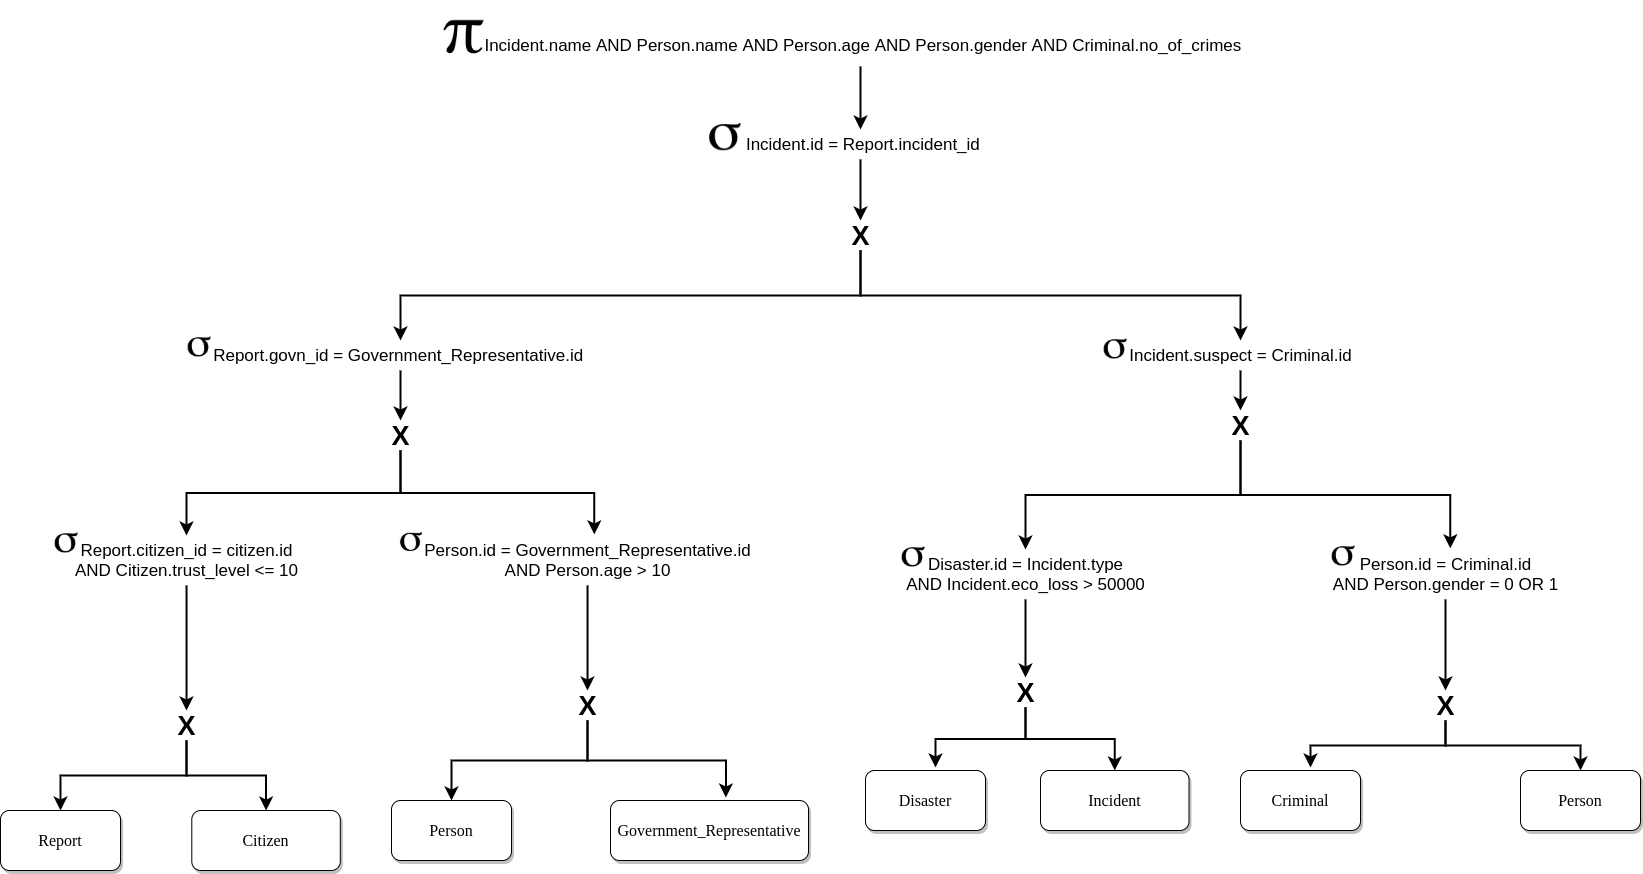
\includegraphics[width=0.8\textwidth]{images/query_trees/query1-non-optimized-initial-version.png}
    \caption{Initial version of query tree for non-optimized query 1}
\end{figure}
\begin{figure}[H]
    \centering
    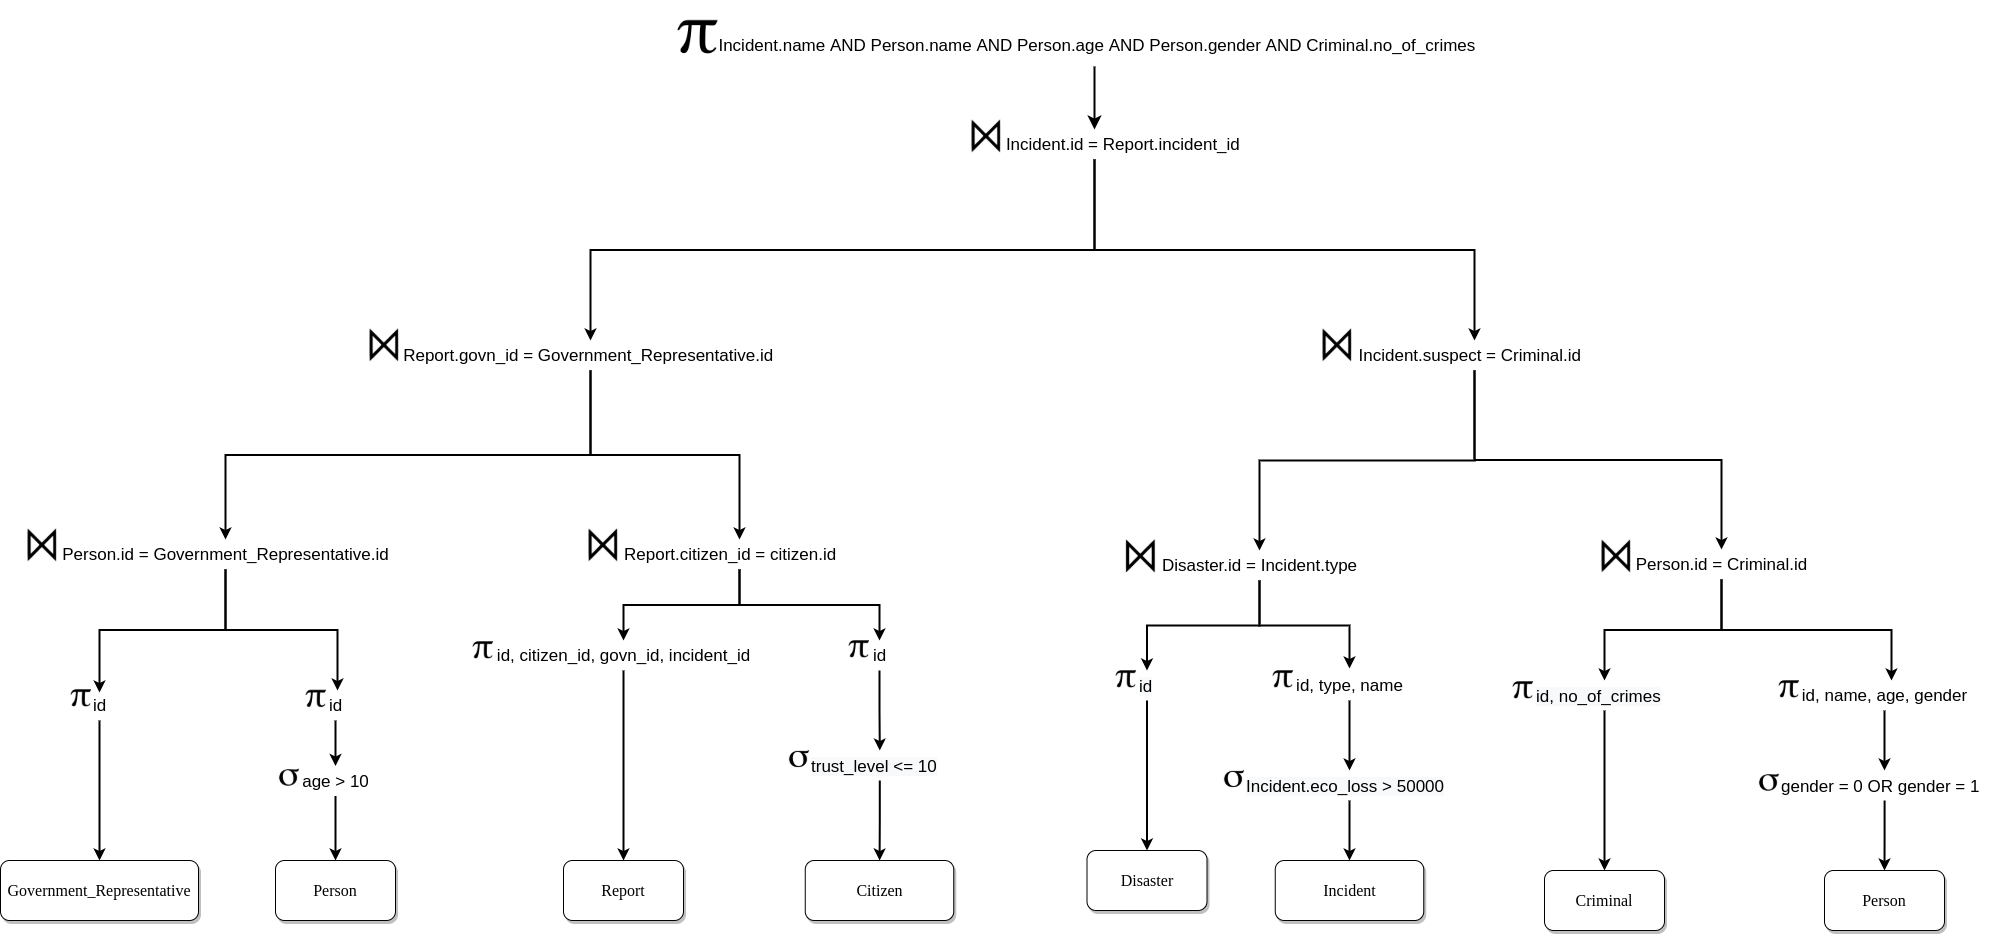
\includegraphics[width=0.8\textwidth]{images/query_trees/query1-non-optimized-final-version.png}
    \caption{Final version of query tree for non-optimized query 1}
\end{figure}
\begin{figure}[H]
    \centering
    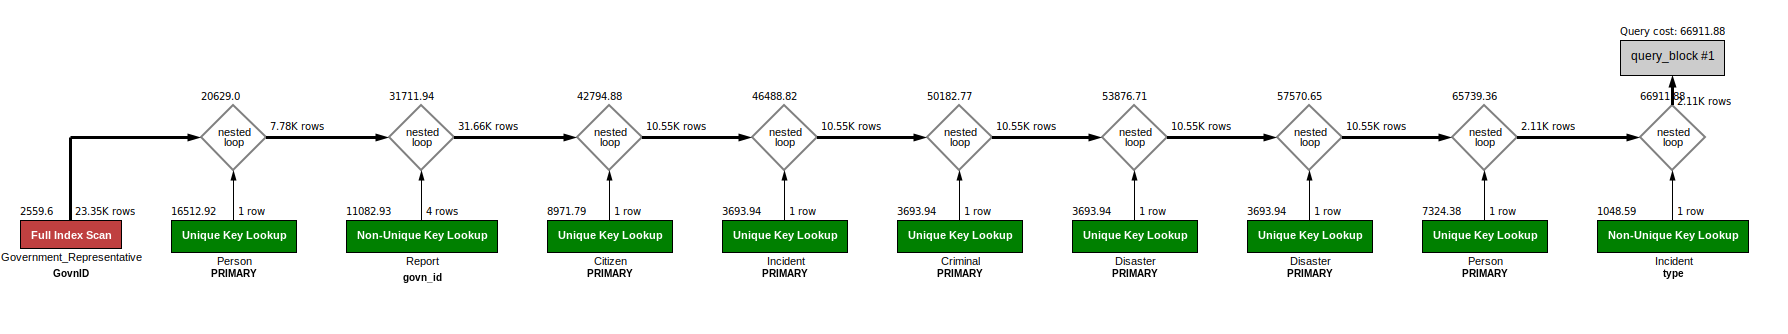
\includegraphics[width=\textwidth]{images/execution_plans/q1-1-old.png}
    \caption{Visual execution plan for non-optimized query 1}
\end{figure}

\subsubsection{Execution Plan After Optimization}
\begin{figure}[H]
    \centering
    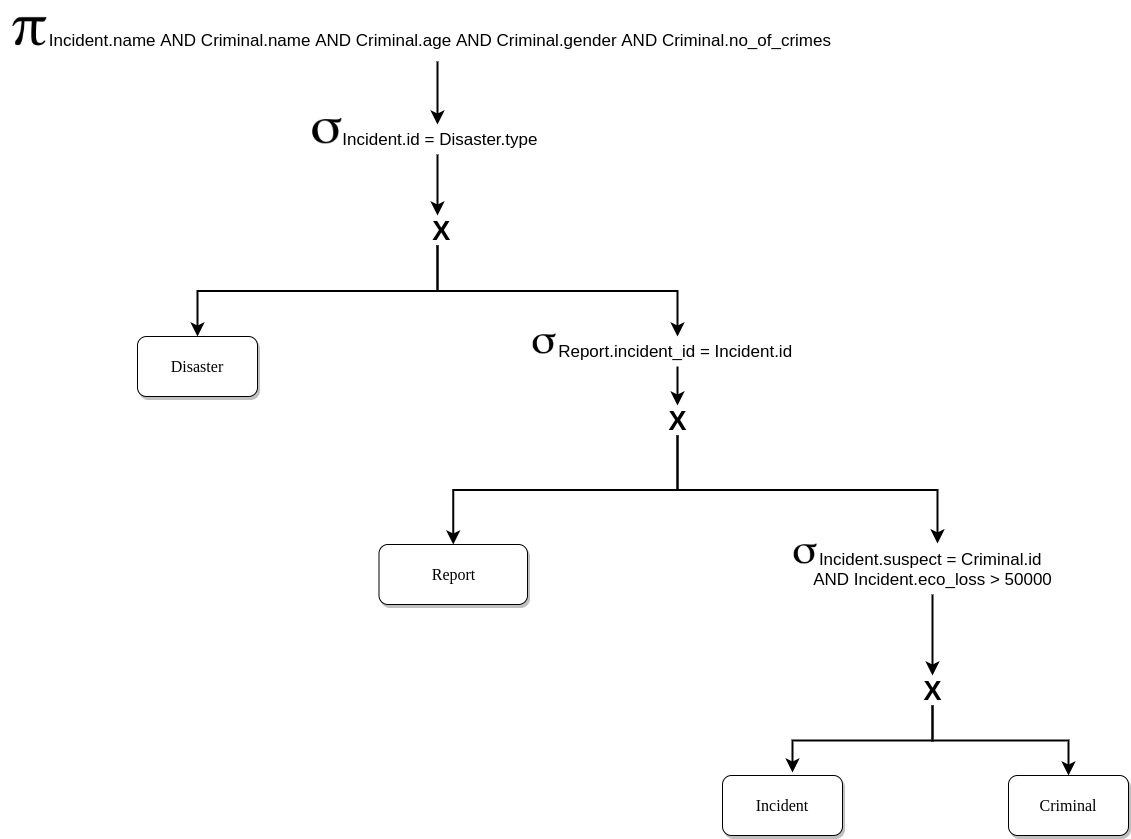
\includegraphics[width=0.8\textwidth]{images/query_trees/query1-optimized-initial-version.png}
    \caption{Initial version of query tree for optimized query 1}
\end{figure}
\begin{figure}[H]
    \centering
    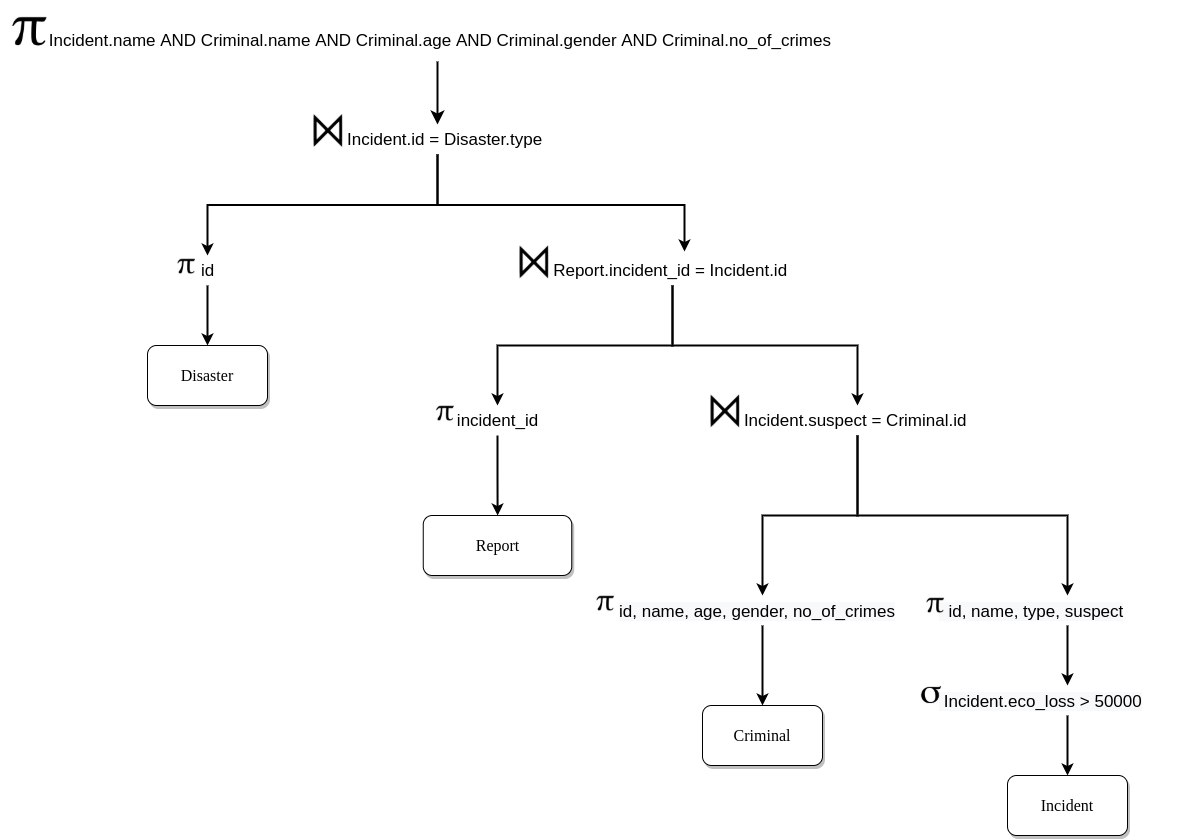
\includegraphics[width=0.8\textwidth]{images/query_trees/query1-optimized-final-version.png}
    \caption{Final version of query tree for optimized query 1}
\end{figure}
\begin{figure}[H]
    \centering
    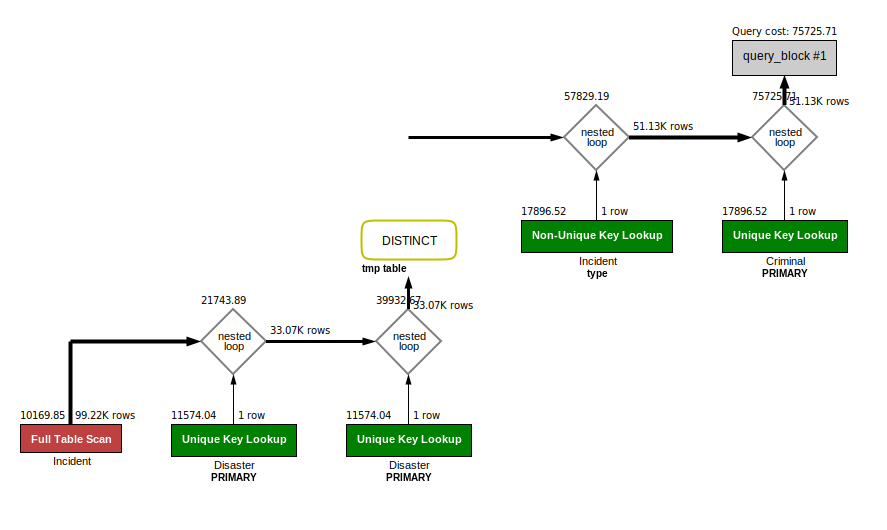
\includegraphics[width=\textwidth]{images/execution_plans/q1-3-new.png}
    \caption{Visual execution plan for optimized query 1}
\end{figure}

\subsubsection{Parallel Query Execution}
We can do the following analysis theoretically :
\begin{itemize}
    \item The \textbf{incident} table is fully scanned through a single worker (thread). Since we are using a \emph{4-core} processor, This scan can be run on 4 threads. The results from 4 streams are, then, gathered into a single stream. This can reduce the full scan time in the previous execution plan to \emph{quarter}.  
\end{itemize}

\subsection{Query 2}

\subsubsection{Execution Plan Before Optimization}
\textbf{Note that,} due to the huge execution time of the query before adding the indexes, we can't extract the actual non-optimized visual execution plan. Therefore, we included the visual execution plan after \emph{index optimization}.
\begin{figure}[H]
    \centering
    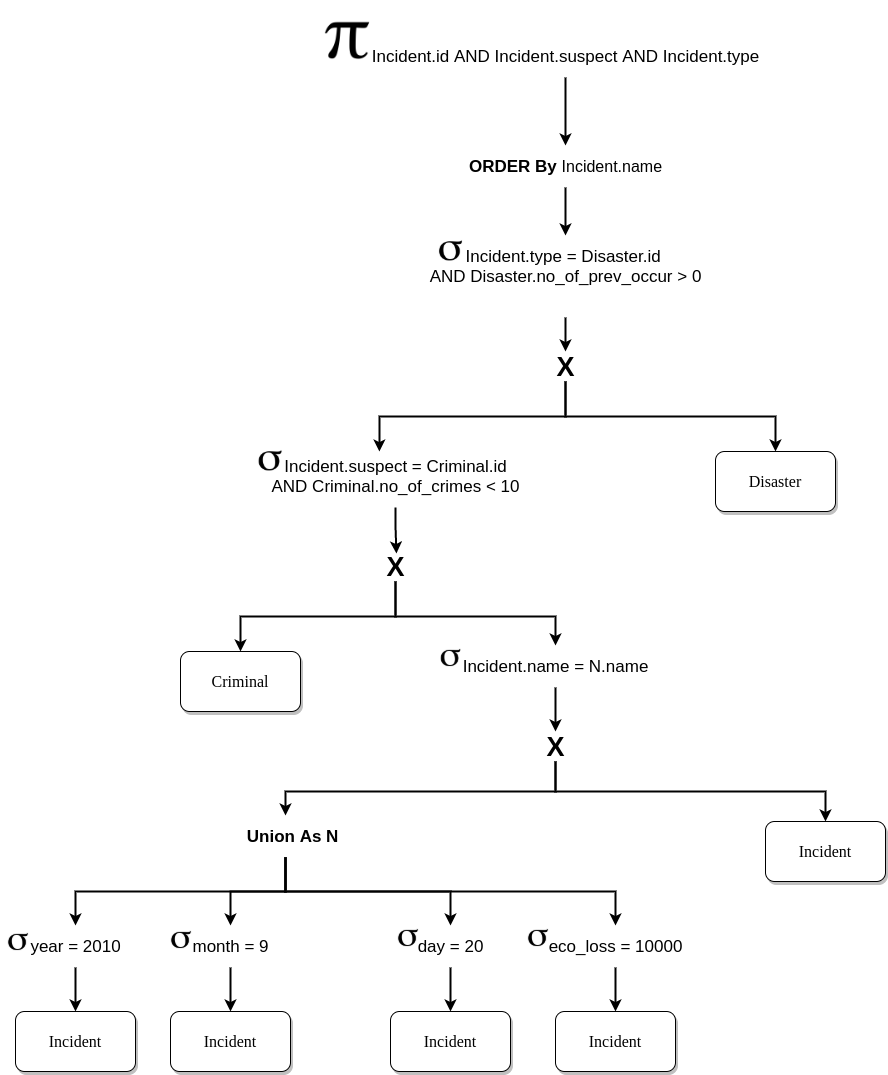
\includegraphics[width=0.8\textwidth]{images/query_trees/query2-non-optimized-initial-version.png}
    \caption{Initial version of query tree for non-optimized query 2}
\end{figure}
\begin{figure}[H]
    \centering
    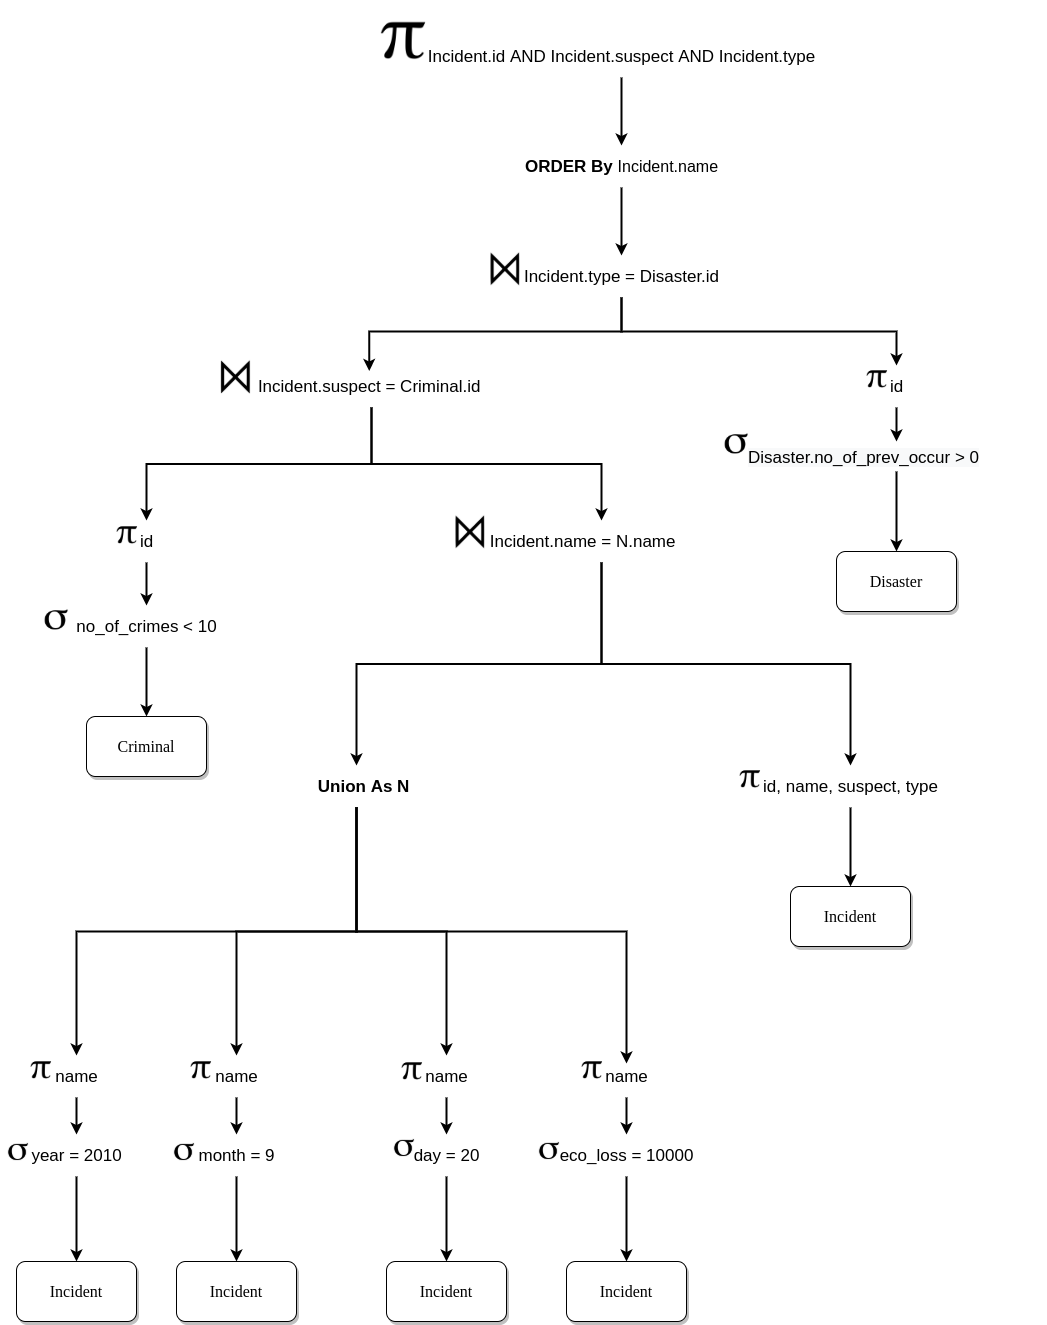
\includegraphics[width=0.8\textwidth]{images/query_trees/query2-non-optimized-final-version.png}
    \caption{Final version of query tree for non-optimized query 2}
\end{figure}
\begin{figure}[H]
    \centering
    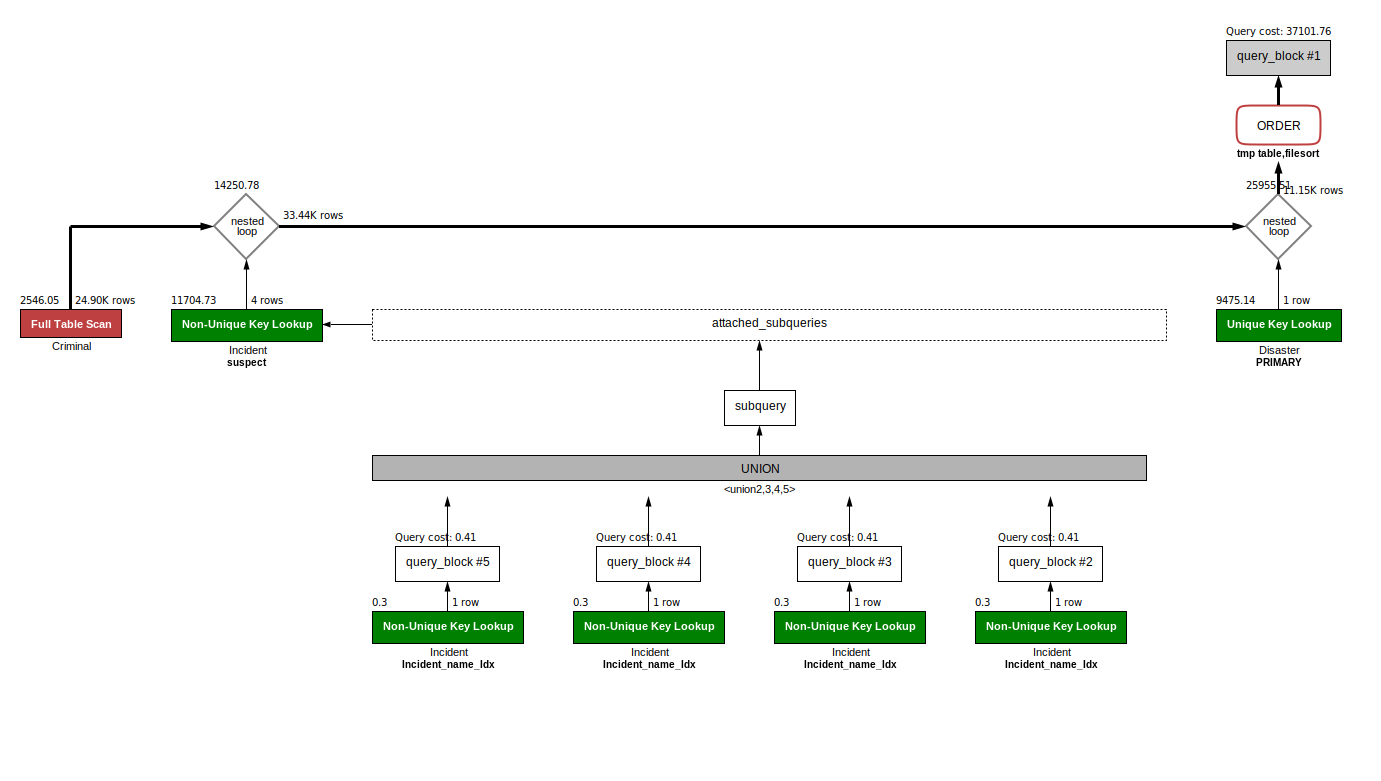
\includegraphics[width=\textwidth]{images/execution_plans/q2-2-new.png}
    \caption{Visual execution plan for non-optimized query 2}
\end{figure}

\subsubsection{Execution Plan After Optimization}
\begin{figure}[H]
    \centering
    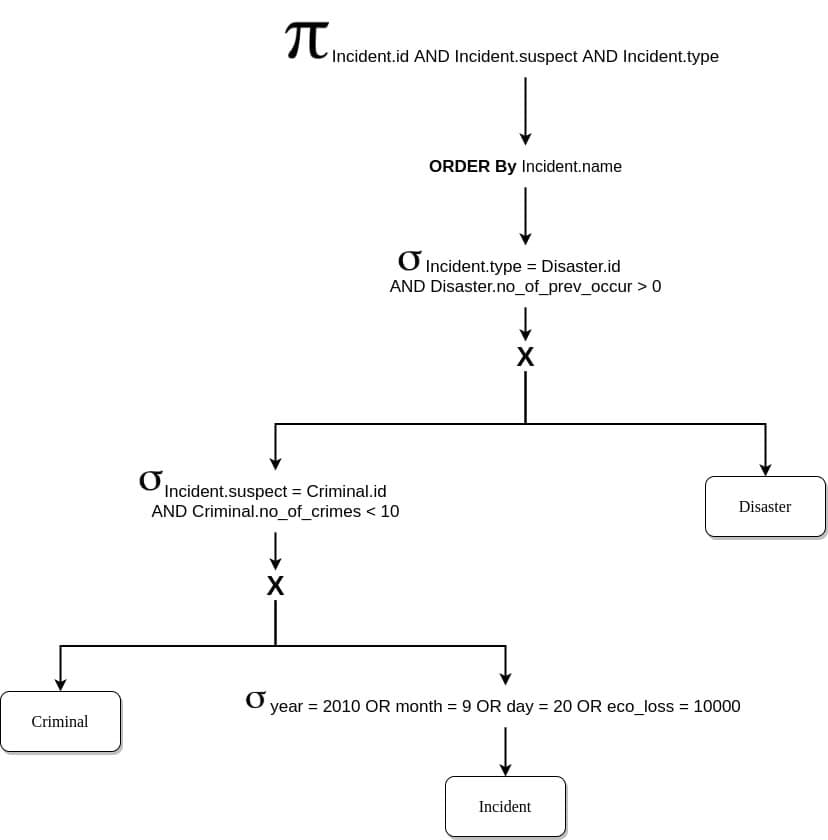
\includegraphics[width=0.8\textwidth]{images/query_trees/query2-optimized-initial-version.png}
    \caption{Initial version of query tree for optimized query 2}
\end{figure}
\begin{figure}[H]
    \centering
    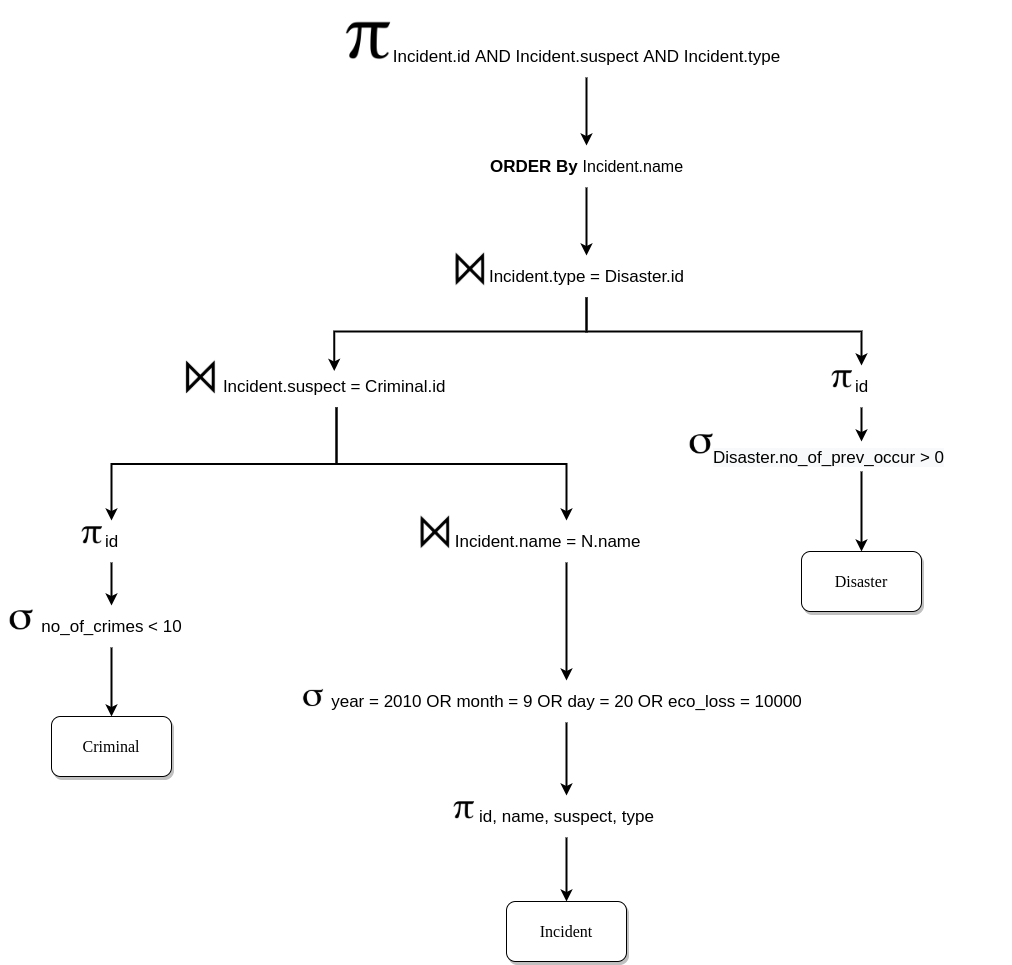
\includegraphics[width=0.8\textwidth]{images/query_trees/query2-optimized-final-version.png}
    \caption{Final version of query tree for optimized query 2}
\end{figure}
\begin{figure}[H]
    \centering
    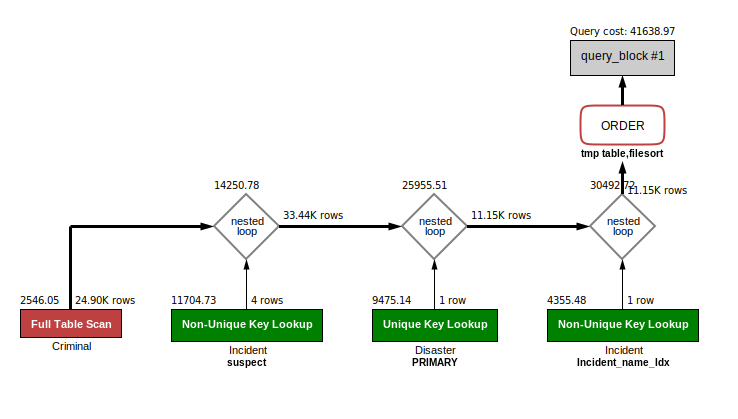
\includegraphics[width=\textwidth]{images/execution_plans/q2-4-new.png}
    \caption{Visual execution plan for optimized query 2}
\end{figure}

\subsubsection{Parallel Query Execution}
We can do the following analysis theoretically :
\begin{itemize}
    \item According to the previous \emph{execution plan}, the \emph{criminal} table is fully scanned at the beginning. This operation is done on a single thread. However, it can be executed in parallel on $4$ threads, which can reduce time to \emph{quarter}. The $4$ previous streams can be gathered in a single stream.
    \item Also, the resulting temporary table is sorted in a single thread. However, it can be done on $4$ threads and then gathered to significantly reduce the costy time of sort.
    \item Also note that using \emph{or} operation is the fastest on a single thread, however using 
    \emph{unions} instead can provide more potential for parallel execution. Each \textbf{union} can be executed on a thread and then gathered to reduce time to \emph{quarter}.
\end{itemize}

\subsection{Query 3}

\subsubsection{Execution Plan Before Optimization}
\begin{figure}[H]
    \centering
    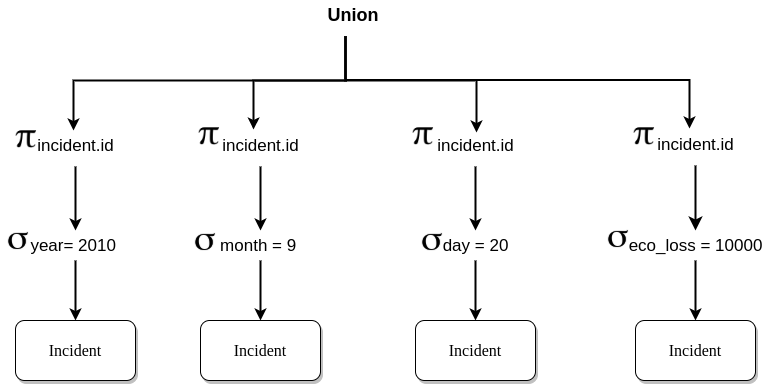
\includegraphics[width=0.8\textwidth]{images/query_trees/query3-optimized-and-non-optimized.png}
    \caption{Query tree for non-optimized query 3}
\end{figure}
\begin{figure}[H]
    \centering
    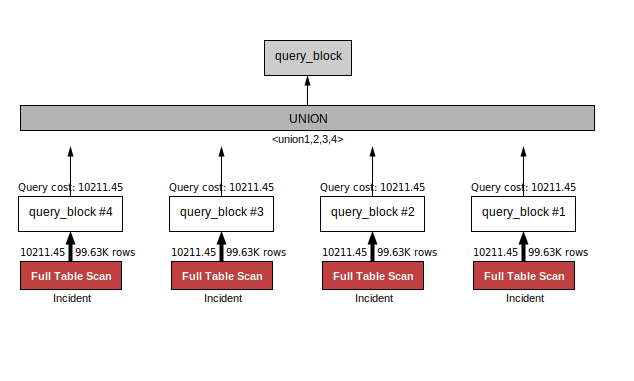
\includegraphics[width=\textwidth]{images/execution_plans/q3-1-old.png}
    \caption{Visual execution plan for non-optimized query 3}
\end{figure}

\subsubsection{Execution Plan After Optimization}
\begin{figure}[H]
    \centering
    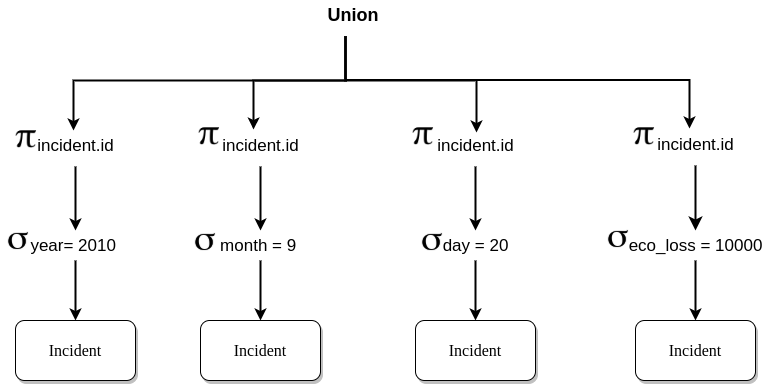
\includegraphics[width=0.8\textwidth]{images/query_trees/query3-optimized-and-non-optimized.png}
    \caption{Query tree for optimized query 3}
\end{figure}
\begin{figure}[H]
    \centering
    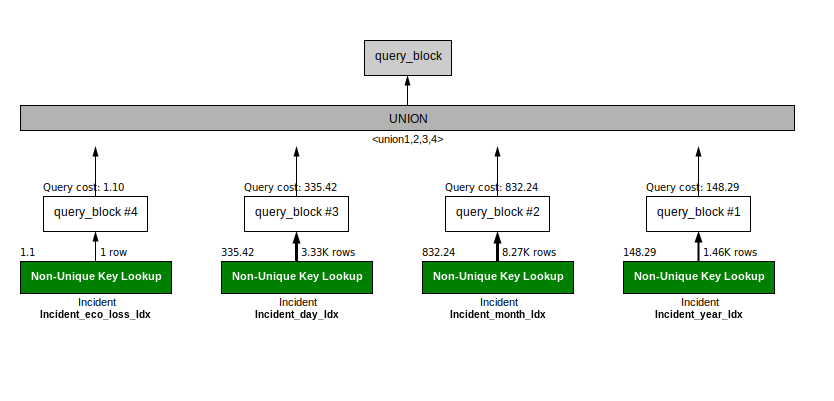
\includegraphics[width=\textwidth]{images/execution_plans/q3-3-new.png}
    \caption{Visual execution plan for optimized query 3}
\end{figure}

\subsubsection{Parallel Query Execution}
We can do the following analysis theoretically :
\begin{itemize}
    \item From the previous \emph{execution plan}, it's obvious that the query can be divided on $4$ threads, one for each \emph{union} operation. The results are, then, gathered from $4$ streams, which allows for time reduction up to \emph{quarter}.
\end{itemize}

\subsection{Query 4}

\subsubsection{Execution Plan Before Optimization}
\begin{figure}[H]
    \centering
    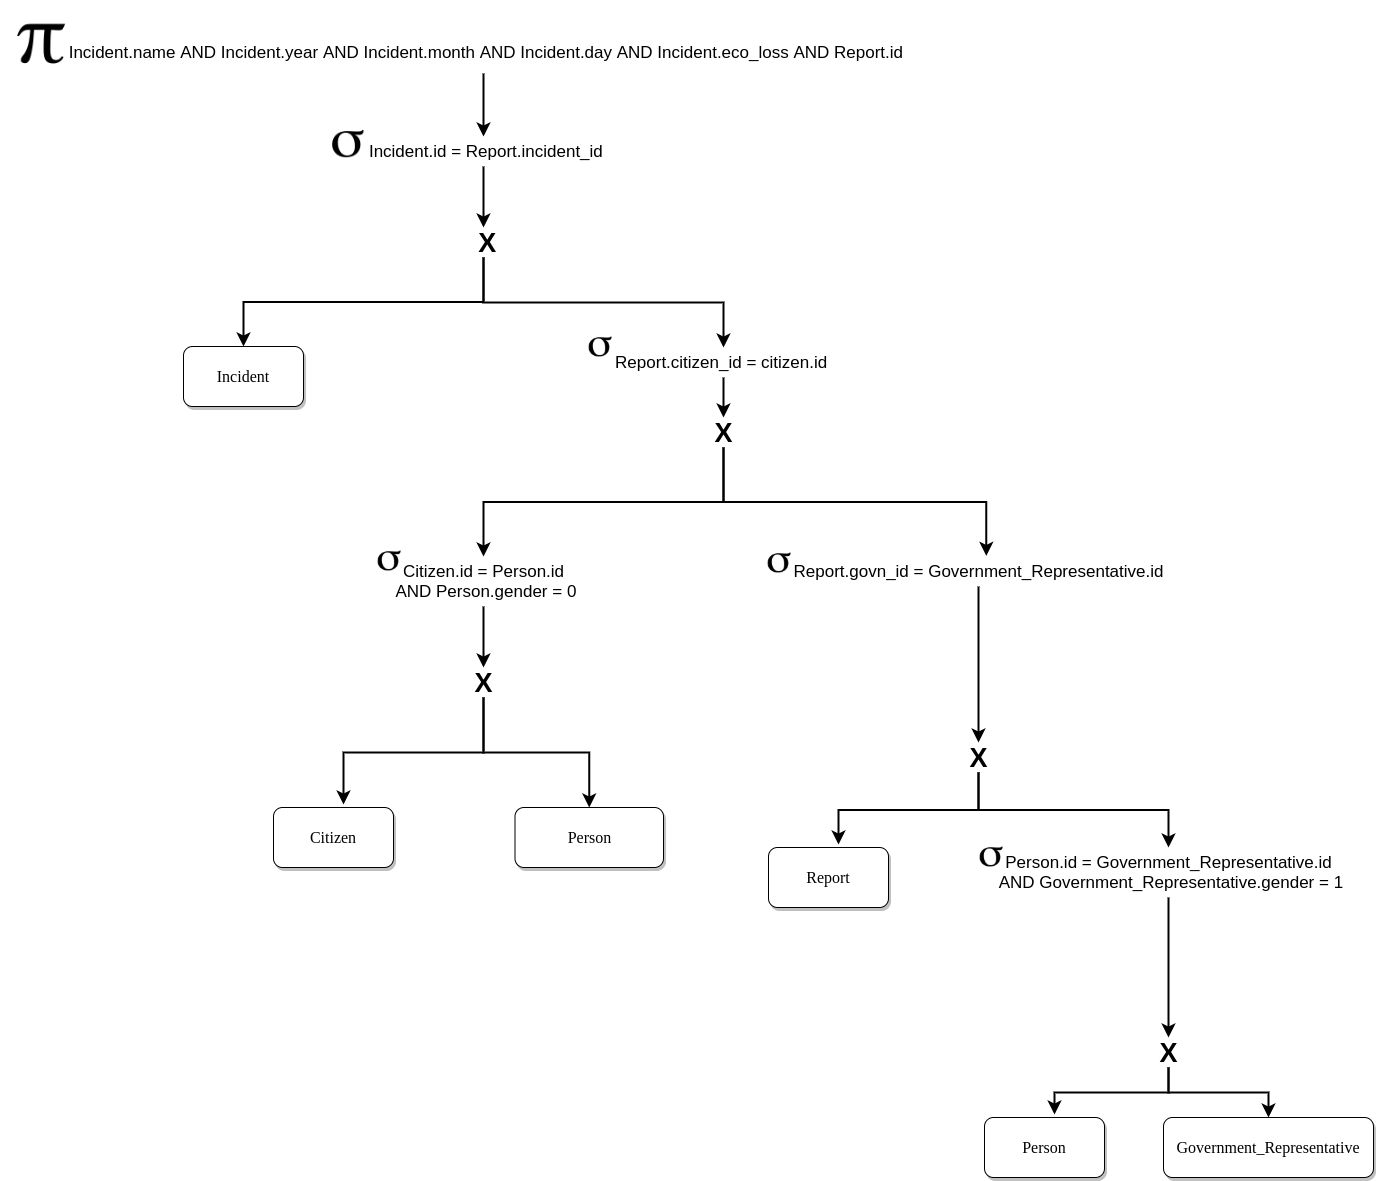
\includegraphics[width=0.8\textwidth]{images/query_trees/query4-non-optimized-initial-version.png}
    \caption{Initial version of query tree for non-optimized query 4}
\end{figure}
\begin{figure}[H]
    \centering
    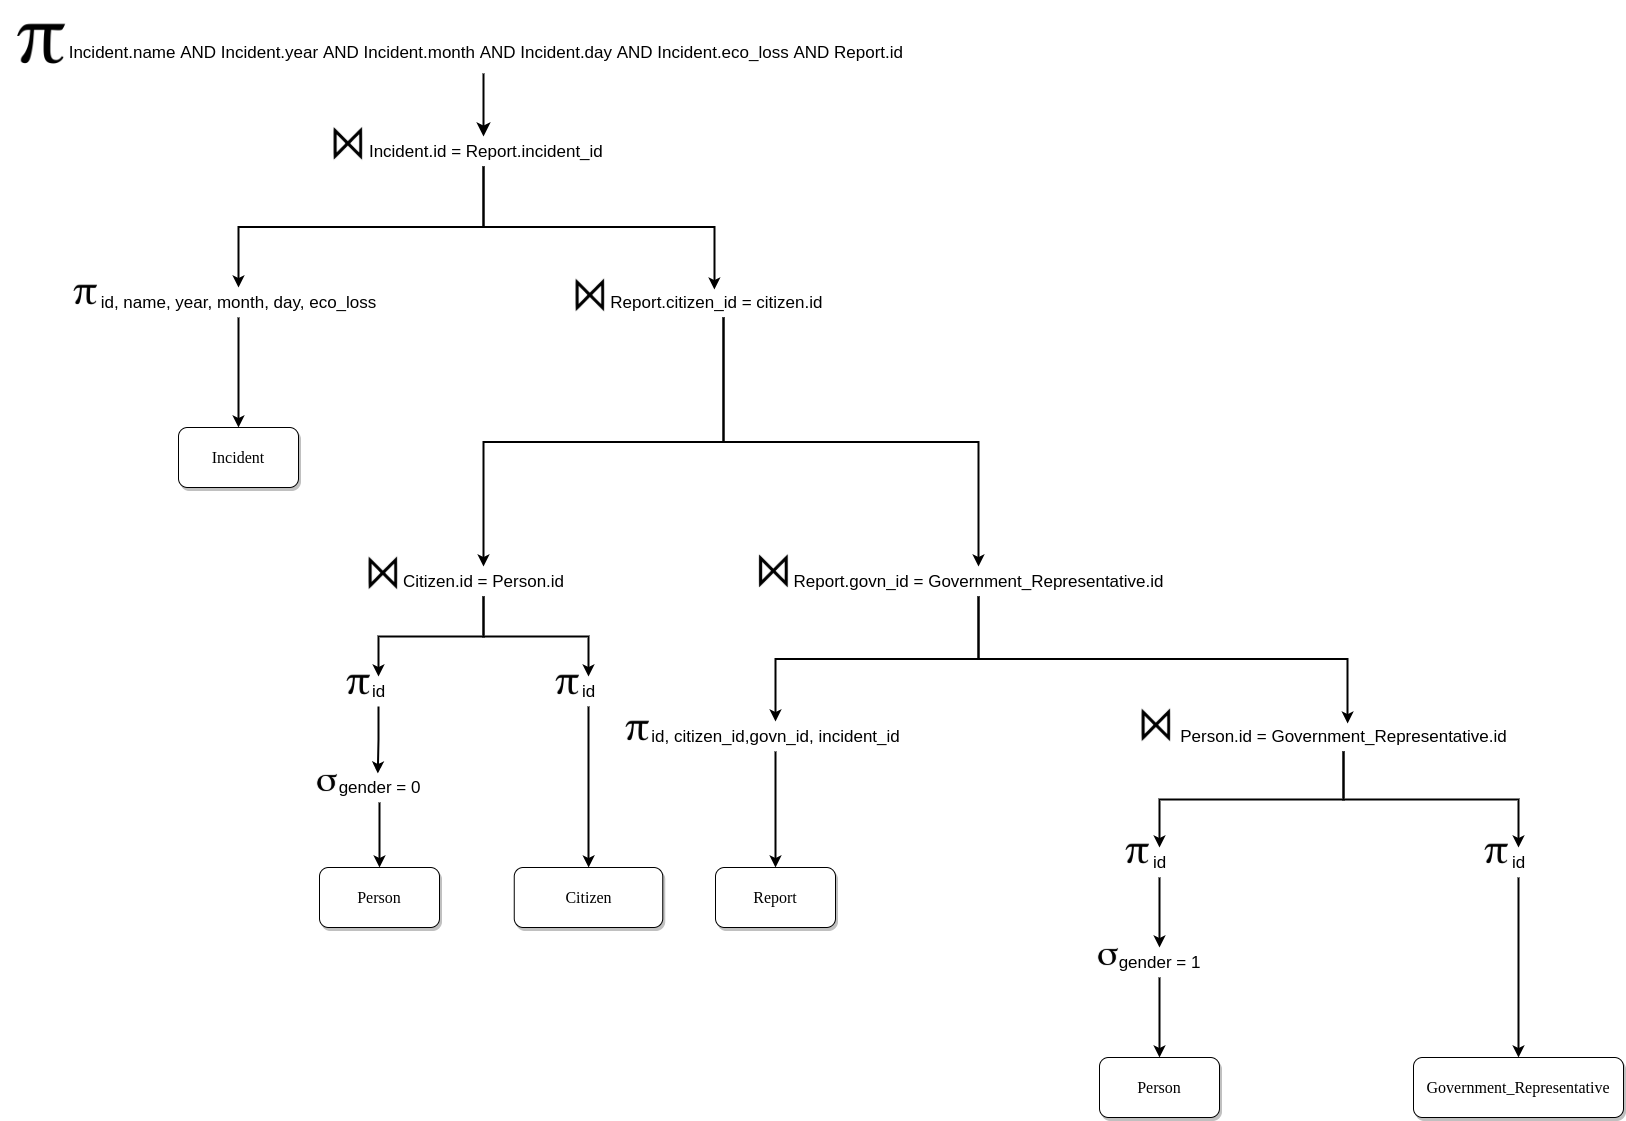
\includegraphics[width=0.8\textwidth]{images/query_trees/query4-non-optimized-final-version.png}
    \caption{Final version of query tree for non-optimized query 4}
\end{figure}
\begin{figure}[H]
    \centering
    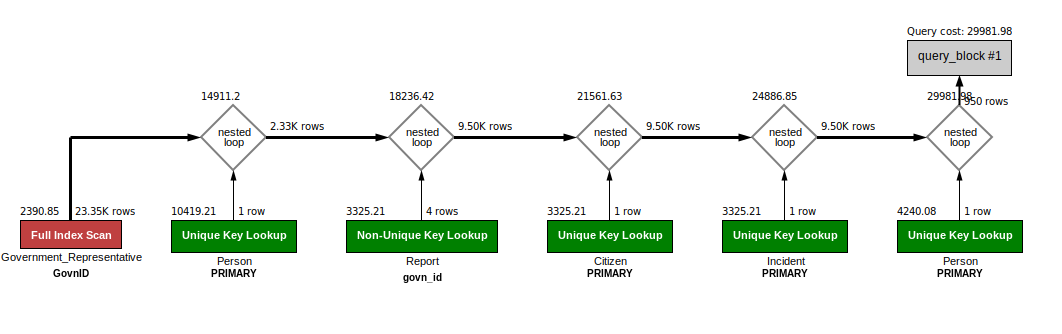
\includegraphics[width=\textwidth]{images/execution_plans/q4-1-old.png}
    \caption{Visual execution plan for non-optimized query 4}
\end{figure}

\subsubsection{Execution Plan After Optimization}
\begin{figure}[H]
    \centering
    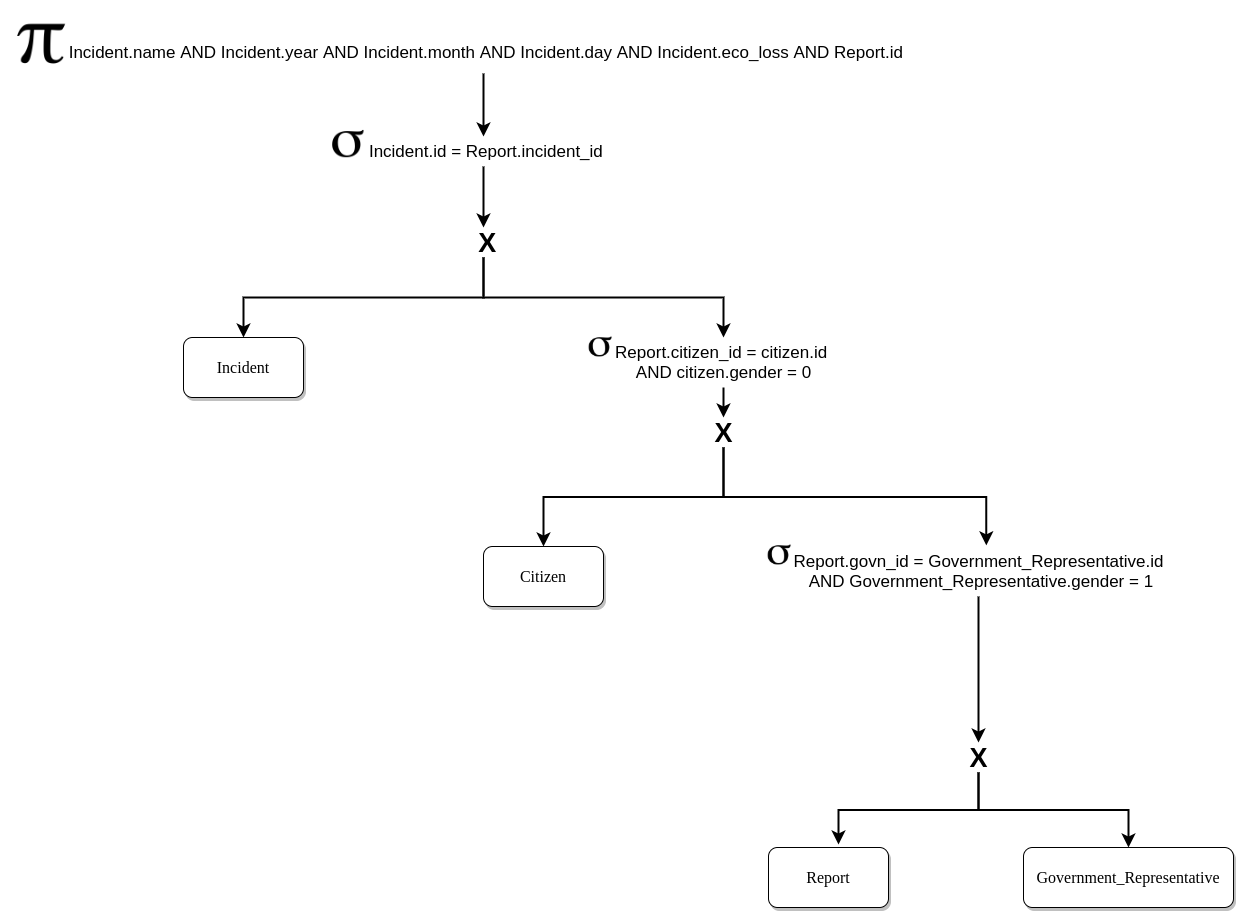
\includegraphics[width=0.8\textwidth]{images/query_trees/query4-optimized-initial-version.png}
    \caption{Initial version of query tree for optimized query 4}
\end{figure}
\begin{figure}[H]
    \centering
    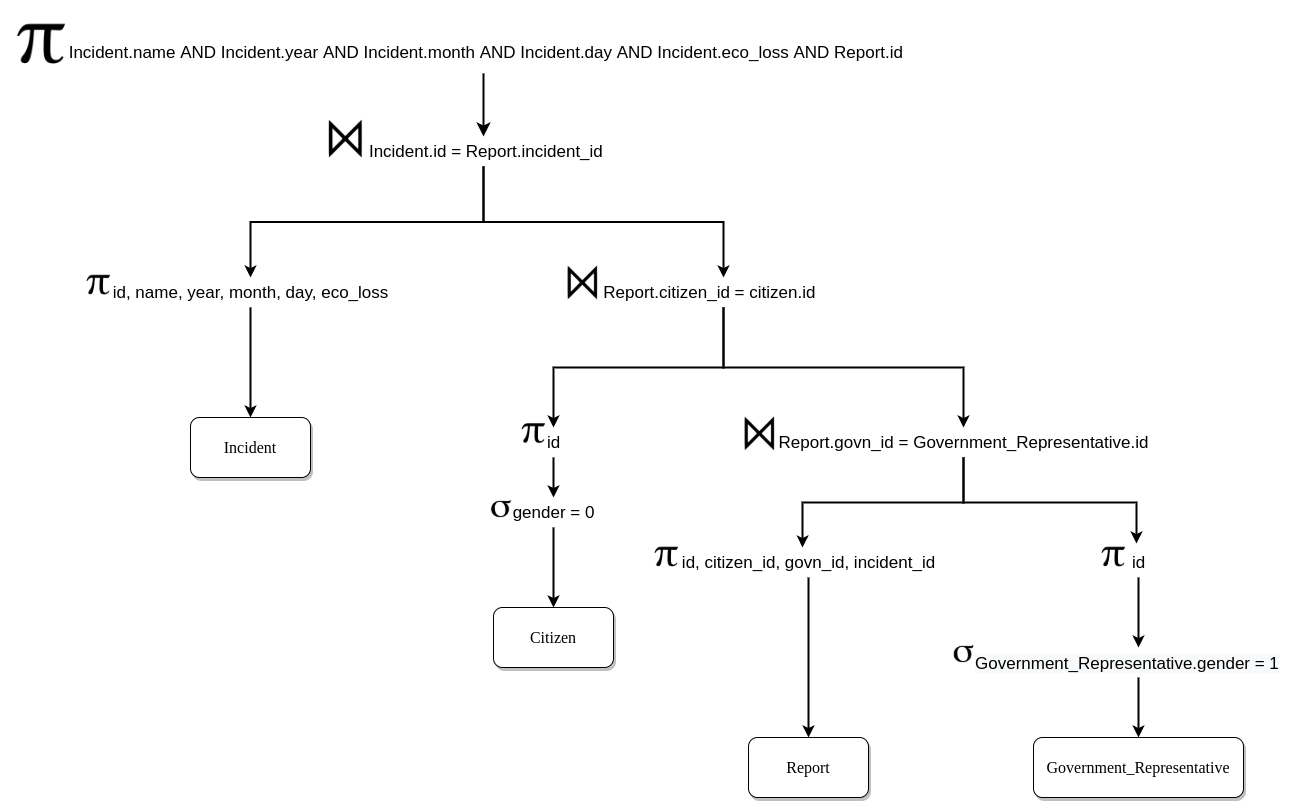
\includegraphics[width=0.8\textwidth]{images/query_trees/query4-optimized-final-version.png}
    \caption{Final version of query tree for optimized query 4}
\end{figure}
\begin{figure}[H]
    \centering
    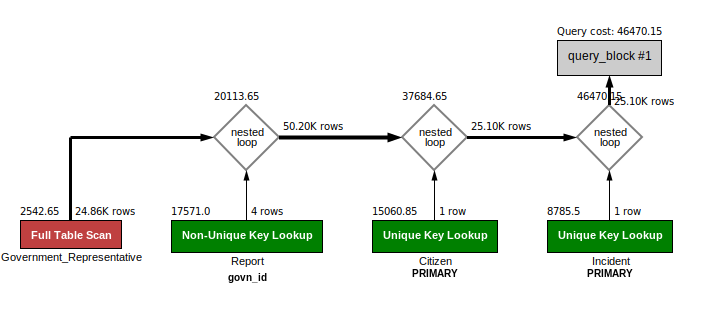
\includegraphics[width=\textwidth]{images/execution_plans/q4-2-new.png}
    \caption{Visual execution plan for optimized query 4}
\end{figure}

\subsubsection{Parallel Query Execution}
We can do the following analysis theoretically :
\begin{itemize}
    \item The \textbf{Government\_Representative} table is fully scanned through a single worker (thread). Since we are using a \emph{4-core} processor, This scan can be run on 4 threads. The results from 4 streams are, then, gathered into a single stream. This can reduce the full scan time in the previous execution plan to \emph{quarter}.
\end{itemize}

\subsection{Query 5}

\subsubsection{Execution Plan Before Optimization}
\begin{figure}[H]
    \centering
    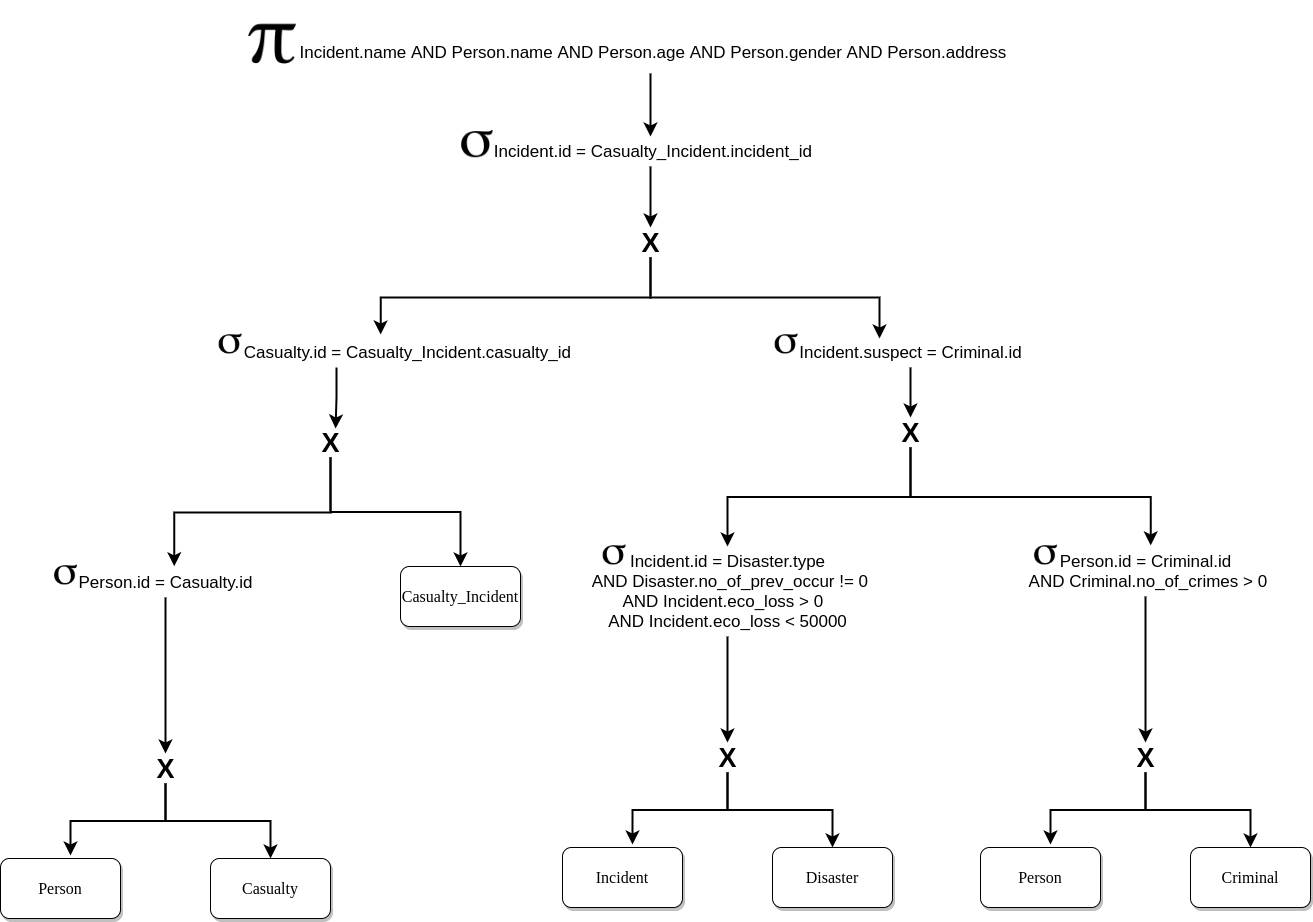
\includegraphics[width=0.8\textwidth]{images/query_trees/query5-non-optimized-initial-version.png}
    \caption{Initial version of query tree for non-optimized query 5}
\end{figure}
\begin{figure}[H]
    \centering
    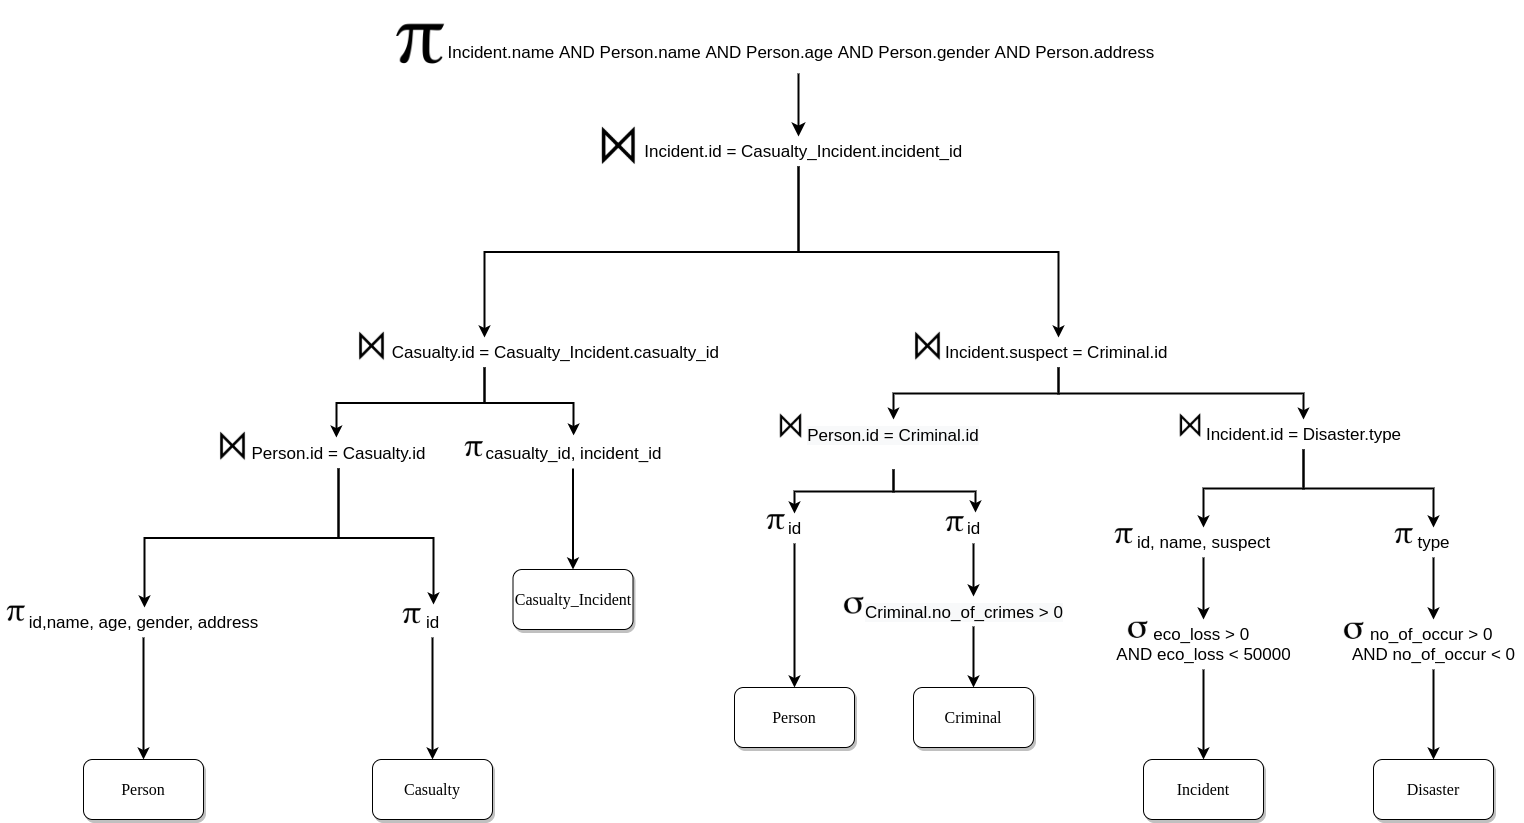
\includegraphics[width=0.8\textwidth]{images/query_trees/query5-non-optimized-final-version.png}
    \caption{Final version of query tree for non-optimized query 5}
\end{figure}
\begin{figure}[H]
    \centering
    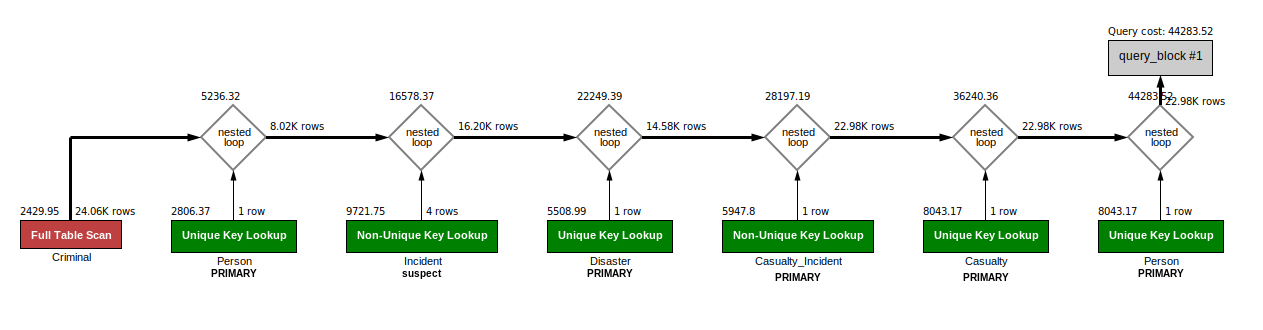
\includegraphics[width=\textwidth]{images/execution_plans/q5-1-old.png}
    \caption{Visual execution plan for non-optimized query 5}
\end{figure}

\subsubsection{Execution Plan After Optimization}
\begin{figure}[H]
    \centering
    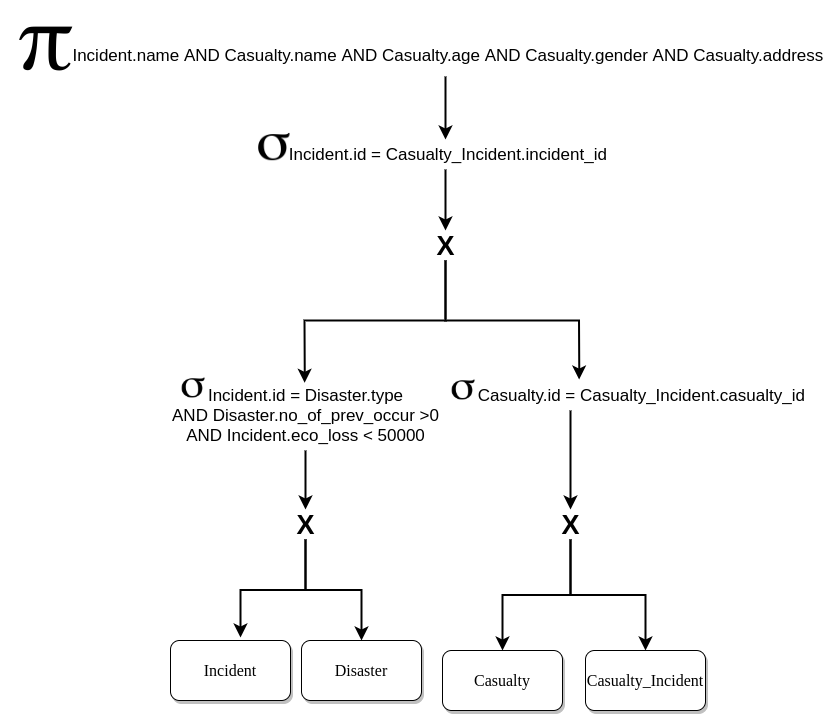
\includegraphics[width=0.8\textwidth]{images/query_trees/query5-optimized-initial-version.png}
    \caption{Initial version of query tree for optimized query 5}
\end{figure}
\begin{figure}[H]
    \centering
    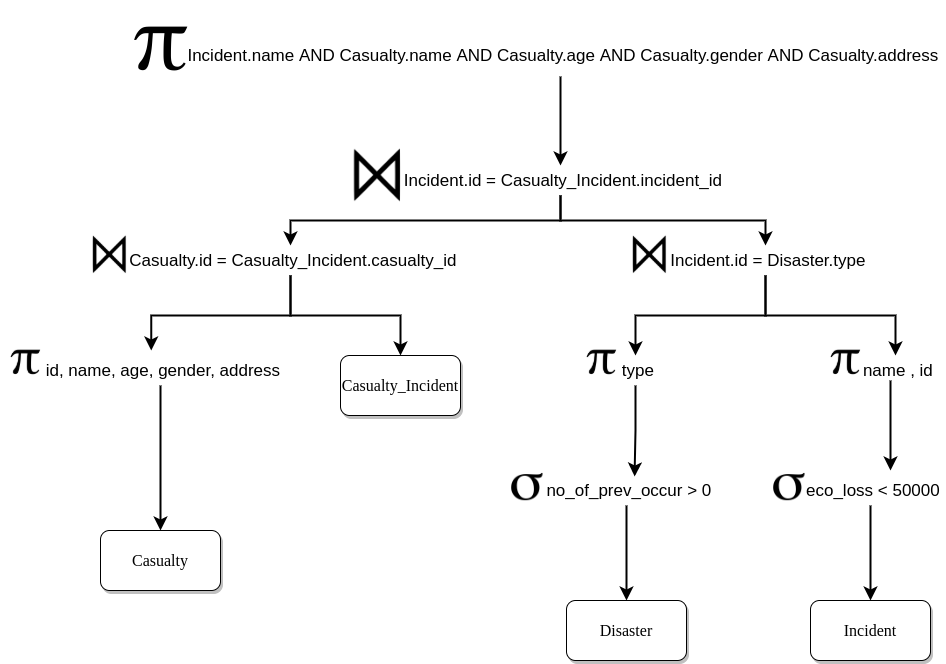
\includegraphics[width=0.8\textwidth]{images/query_trees/query5-optimized-final-version.png}
    \caption{Final version of query tree for optimized query 5}
\end{figure}
\begin{figure}[H]
    \centering
    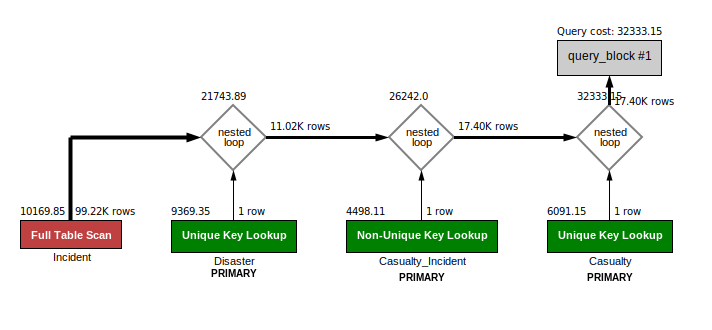
\includegraphics[width=\textwidth]{images/execution_plans/q5-4-new.png}
    \caption{Visual execution plan for optimized query 5}
\end{figure}

\subsubsection{Parallel Query Execution}
We can do the following analysis theoretically :
\begin{itemize}
    \item The \textbf{incident} table is fully scanned through a single worker (thread). We can see from the estimated cost that this takes up most of the query time. Since we are using a \emph{4-core} processor, This scan can be run on 4 threads. The results from 4 streams are, then, gathered into a single stream. This can reduce the full scan time in the previous execution plan to \emph{quarter}. This will greatly affect the query execution time.
\end{itemize}